
\documentclass{article}
\usepackage[T1]{fontenc}
\usepackage[utf8]{inputenc}
\usepackage[spanish]{babel}
\usepackage{amssymb, amsmath, amsbsy} % simbolitos
\usepackage{graphicx}
\title{Práctica 1\\Algoritmos paralelos}
\author{Peto Gutierrez Emmanuel}
\begin{document}
\maketitle

Los tiempos de ejecución se dan en microsegundos.

\begin{table}[h]
\begin{tabular}{|c|c|c|c|c|c|c|}
\hline
\textbf{Hilos} & \textbf{Promedio} & \textbf{Prueba 1} & \textbf{Prueba 2} & \textbf{Prueba 3} & \textbf{Prueba 4} & \textbf{Prueba 5}\\
\hline
\textbf{1} & 3260610.8 & 2909366 & 3008953 & 3499814 & 3399712 & 3485209 \\
\hline
\textbf{2} & 1800342.2 & 1802146 & 1803782 & 1802388 & 1800056 & 1793339 \\
\hline
\textbf{4} & 1003428.2 & 1000947 & 1004894 & 1002809 & 1008122 & 1000369 \\
\hline
\textbf{6} & 1006349 & 1004090 & 985663 & 985174 & 1037144 & 1019674 \\
\hline
\textbf{8} & 994660.8 & 973975 & 1033171 & 987956 & 996128 & 982074 \\
\hline
\textbf{20} & 1008209 & 1004286 & 1008287 & 1006698 & 1013719 & 1008055 \\
\hline
\textbf{50} & 1021020.6 & 1019131 & 1019676 & 1027698 & 1022113 & 1016485 \\
\hline
\textbf{100} & 1030163.6 & 1032759 & 1032854 & 1029508 & 1027225 & 1028472 \\
\hline
\end{tabular}
\caption{Tabla de tiempos de ejecución. Primera ejecución.}
\label{table:1}
\end{table}

\begin{table}[h]
\begin{tabular}{|c|c|c|c|c|c|c|}
\hline
\textbf{Hilos} & \textbf{Promedio} & \textbf{Prueba 1} & \textbf{Prueba 2} & \textbf{Prueba 3} & \textbf{Prueba 4} & \textbf{Prueba 5}\\
\hline
\textbf{1} & 3149860.6 & 3141505 & 3138417 & 3168281 & 3136131 & 3164969 \\
\hline
\textbf{2} & 1668833.8 & 1714920 & 1653986 & 1645437 & 1642501 & 1687325 \\
\hline
\textbf{4} & 1446799.6 & 1426221 & 1386805 & 1414880 & 1491961 & 1514131 \\
\hline
\textbf{6} & 1406982 & 1423169 & 1421549 & 1428480 & 1367871 & 1393841 \\
\hline
\textbf{8} & 1412858.2 & 1392294 & 1428376 & 1353914 & 1418279 & 1471428 \\
\hline
\textbf{20} & 1448111.6 & 1471741 & 1464537 & 1430041 & 1412378 & 1461861 \\
\hline
\textbf{50} & 1457669.8 & 1481467 & 1479378 & 1407743 & 1480156 & 1439605 \\
\hline
\textbf{100} & 1475008.6 & 1489538 & 1496705 & 1466845 & 1477180 & 1444775 \\
\hline
\end{tabular}
\caption{Tabla de tiempos de ejecución. Segunda ejecución.}
\label{table:2}
\end{table}

En el Cuadro \ref{table:1} se muestran los tiempos de ejecución al calcular la suma de los primeros $10^9$ números naturales de forma paralela. Al realizar las ejecuciones no se estaba ejecutando ningún otro proceso en el equipo (salvo por los del sistema operativo).

En el Cuadro \ref{table:2} se muestran los tiempos al calcular la misma suma pero teniendo en ejecución el programa \texttt{cod01.c}.

El equipo donde se ejecutó el programa tiene 4 procesadores con 2 núcleos.

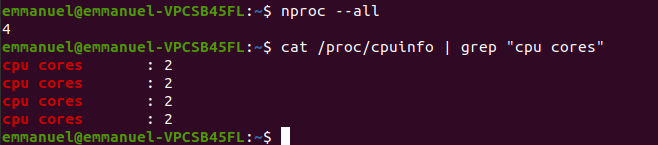
\includegraphics[width=\linewidth]{cores.png}

\vspace{5mm}

En el Cuadro \ref{table:1} se puede observar que ejecutar el programa de forma secuencial toma 3.2 s, ejecutarlo con 2 hilos toma 1.8 s y ejecutarlo con 4 y 6 hilos toma un poco más de 1 s.

El mejor tiempo se obtiene cuando se ejecuta el programa con 8 hilos, con un promedio de 994660.8 $\mu$s (un poco menos de 1 s). Esto es porque se aprovechan los 8 núcleos disponibles.

Cuando se lanzan más de 8 hilos toma más tiempo en ejecutarse que con 8 porque el sistema operativo tiene que asignarle cierto tiempo de CPU a cada hilo hasta que se terminen de ejecutar, pero alternando las ejecuciones entre los procesadores disponibles. Es decir, cambiar de un hilo a otro hace que se pierda un poco de tiempo.

Dados los valores del Cuadro \ref{table:2} se observa que con 1 o 2 hilos no se obtuvo una gran diferencia en el desempeño respecto al Cuadro \ref{table:1}. A partir de 4 hilos se observa que el tiempo de ejecución es mayor que en el Cuadro 1, obtieniendo un mínimo aproximado de 1.4 s. Esto se debe a que algunos procesadores están ocupados ejecutando el programa \texttt{cod01.c}.

\begin{table}
\begin{center}
\begin{tabular}{|l|l|}
\hline
Marca de equipo & Vaio \\ \hline
Sistema operativo & Ubuntu 20.04.2 LTS \\ \hline
Procesador & Intel Core i5-2450M \\ \hline
Generación & 2 \\ \hline
Núcleos & 2 \\ \hline
Mejor tiempo & 994660.8 $\mu$s \\ \hline
nº hilos & 8 \\ \hline
\end{tabular}
\caption{Información de la computadora.}
\end{center}
\end{table}

\end{document}

